\documentclass[12pt]{article}

% TEMPLATE DEFAULT PACKAGES
\usepackage{amssymb,amsmath,amsfonts,eurosym,geometry,ulem,graphicx,color,setspace,sectsty,comment,natbib,pdflscape,array,adjustbox}

% ADDED PACKAGES FOR THIS MANUSCRIPT
\usepackage{palatino,newtxmath,multirow,titlesec,threeparttable,tabu,booktabs,titlesec,threeparttable,mathtools,bm,bbm,subcaption,pdflscape,tcolorbox,mathrsfs,tikz,graphicx}
% endfloat,

\usepackage{afterpage}
\usepackage[hyphens]{url}
\usepackage[margin=1cm]{caption}

\usepackage[draft]{hyperref}
\newcommand{\tim}{$\,\times\,$}
% FIGURES & TABLES CAPTION STYLING
\captionsetup[figure]{labelfont={bf},name={Figure},labelsep=period}
\captionsetup[table]{labelfont={bf},name={Table},labelsep=period}

% SECTION TITLE SETTINGS
\titlelabel{\thetitle.\enskip}
\titleformat*{\section}{\large\bfseries}
\titleformat*{\subsection}{\normalsize\bfseries}

% COLUMN TYPES
\newcolumntype{L}[1]{>{\raggedright\let\newline\\\arraybackslash\hspace{0pt}}m{#1}}
\newcolumntype{C}{>{\centering\arraybackslash}p{5.2em}}
\newcolumntype{D}{>{\centering\arraybackslash}p{5em}}
\newcolumntype{R}[1]{>{\raggedleft\let\newline\\\arraybackslash\hspace{0pt}}m{#1}}


% MARGINS AND SPACING
\normalem
\geometry{left=1.1in,right=1.1in,top=1.0in,bottom=1.0in}
\setlength{\parskip}{2.5pt}

% SPECIAL CELL 
\newcommand{\specialcell}[2][c]{%
	\begin{tabular}[#1]{@{}l@{}}#2\end{tabular}}

% NO INDENT ON FOOTNOTES
\usepackage[hang,flushmargin]{footmisc}

\begin{document}

\section{New Overlap Approach}
\begin{figure*}
        %\vspace{2mm}
        \begin{subfigure}[b]{0.495\textwidth}
            \centering
            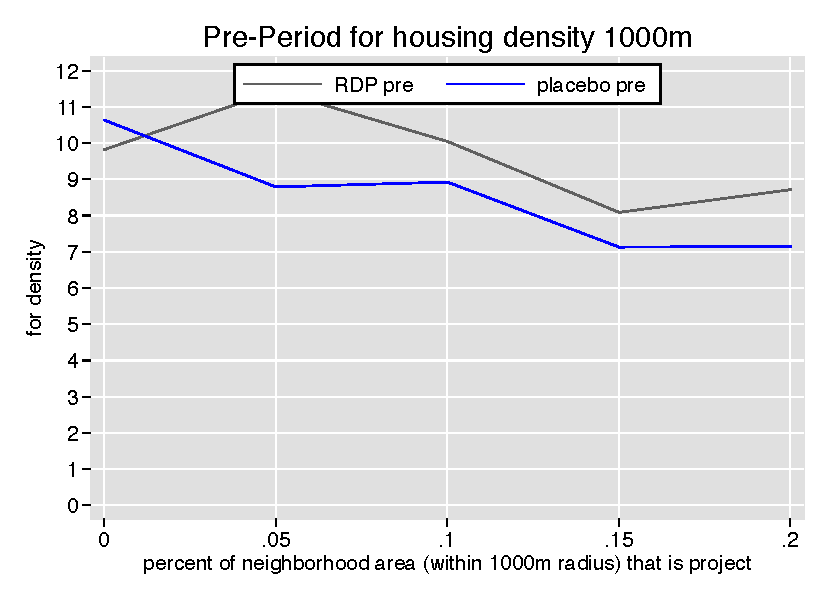
\includegraphics[width=\textwidth,trim={0.3cm .3cm 0.1cm 0cm}, clip=true]{figures/overlap_for_1000_total_pre.pdf}
        \end{subfigure}
        \hfill
        \begin{subfigure}[b]{0.495\textwidth}  
            \centering 
            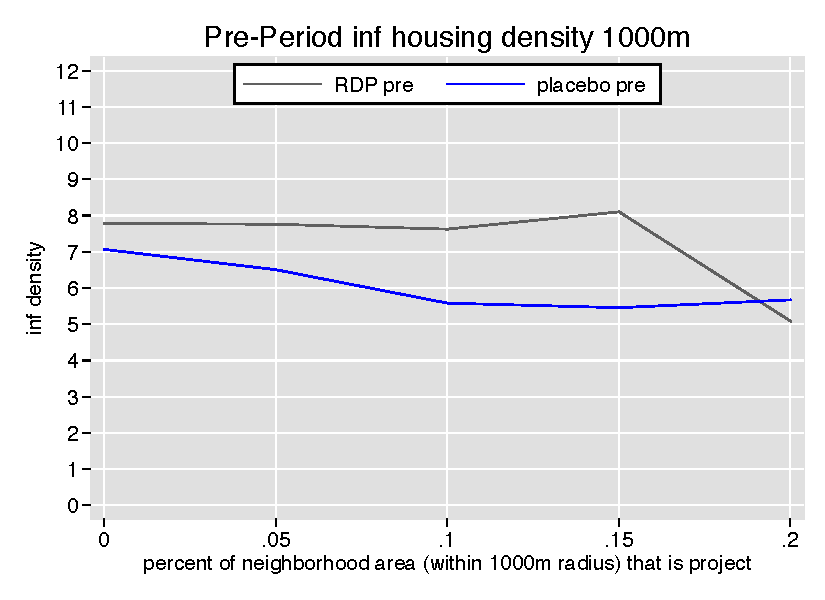
\includegraphics[width=\textwidth,trim={0.3cm .3cm 0.1cm 0cm}, clip=true]{figures/overlap_inf_1000_total_pre.pdf}
        \end{subfigure}
        \vspace{-6mm}
        %\vspace{2mm}
        \begin{subfigure}[b]{0.495\textwidth}
            \centering
            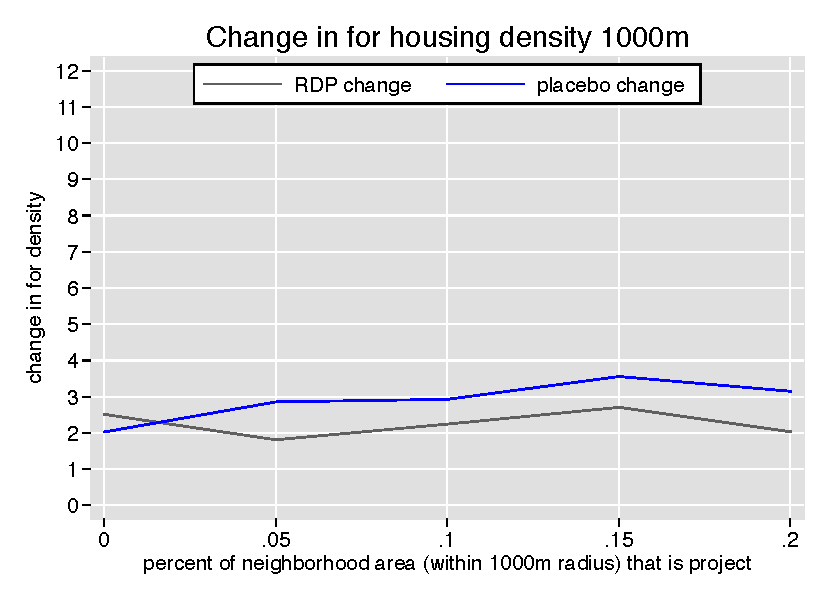
\includegraphics[width=\textwidth,trim={0.3cm .3cm 0.1cm 0cm}, clip=true]{figures/change_for_1000_total.pdf}
        \end{subfigure}
        \hfill
        \begin{subfigure}[b]{0.495\textwidth}  
            \centering 
            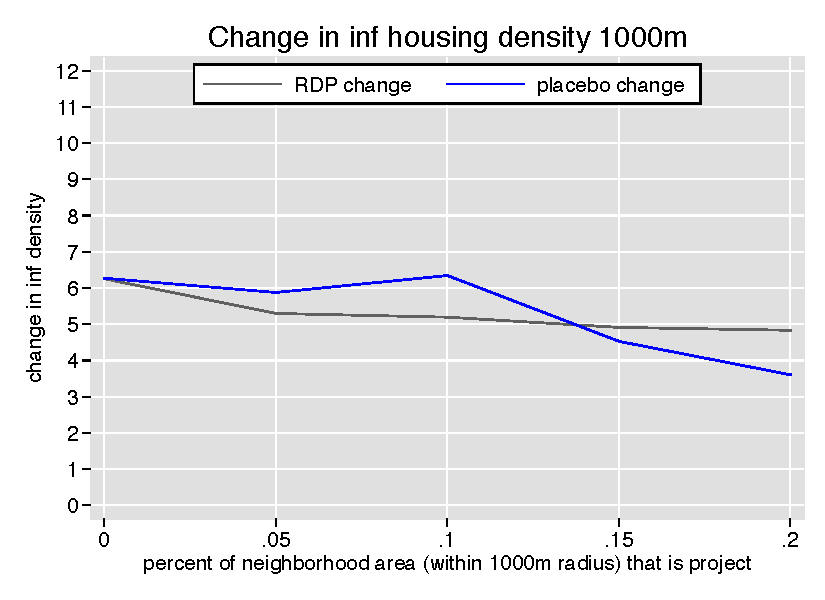
\includegraphics[width=\textwidth,trim={0.3cm .3cm 0.1cm 0cm}, clip=true]{figures/change_inf_1000_total.pdf}
        \end{subfigure}
        \vspace{-6mm}
    \end{figure*} 

\begin{itemize}
	\item how it's made
	\begin{itemize} 
		\item for each 100$\text{m}^{2}$ bblu cell, find the 1km buffer around its centroid
		\item calculate the percentage area overlap between the buffer and RDP and Placebo project areas
		\item the plots above are generated by taking the percent overlap, trimming out the top 5\% of percent overlap (because there is a long weird tail), then plotting averages
	\end{itemize}
	\item why i like it
	\begin{itemize}
		\item i think that's what people care about ``there are a lot of public houses in my neighborhood'' instead of ``the closest public house to me happens to be X meters''
		\item econ theory
		\begin{itemize}
			\item nearest distance might matter for jobs and schools where you have to commute each day
			\item number of public houses in a neighborhood may matter more for disease, congestion, use of public services, ie. maybe more like mechanisms we're interested in 
		\end{itemize}
		\item observations with a lot of projects around them get weighted up, observations on the outskirts get weighted down
		\item big projects have a bigger impact, and since these projects are grids of houses/entire neighborhoods, they probably should
        \item empirically, the plots above have closer baseline means between 
	\end{itemize}
    \item why i don't like it
\end{itemize}




\pagebreak


\section{ROBUSTNESS : vary all the bandwidths}


\begin{figure*}
        %\vspace{2mm}
        \begin{subfigure}[b]{0.495\textwidth}
            \centering
            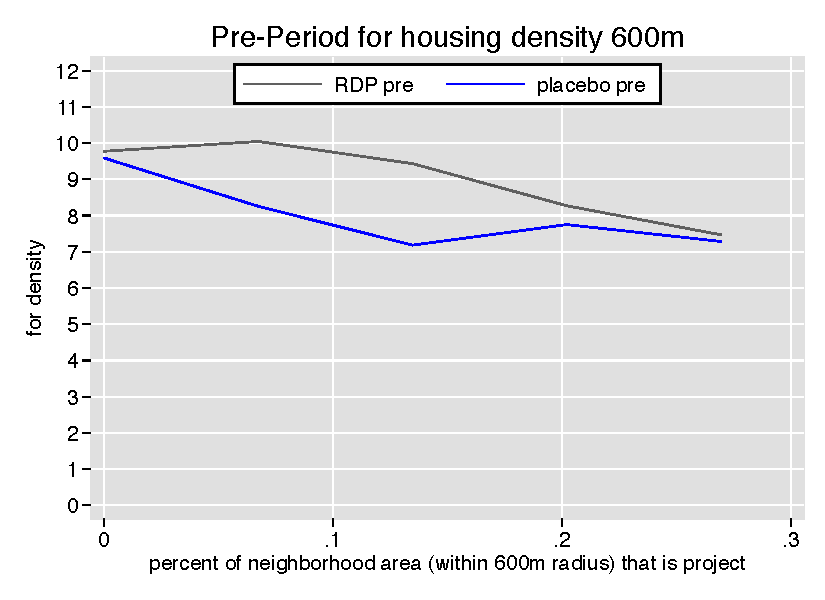
\includegraphics[width=\textwidth,trim={0.3cm .3cm 0.1cm 0cm}, clip=true]{figures/overlap_for_600_total_pre.pdf}
        \end{subfigure}
        \hfill
        \begin{subfigure}[b]{0.495\textwidth}  
            \centering 
            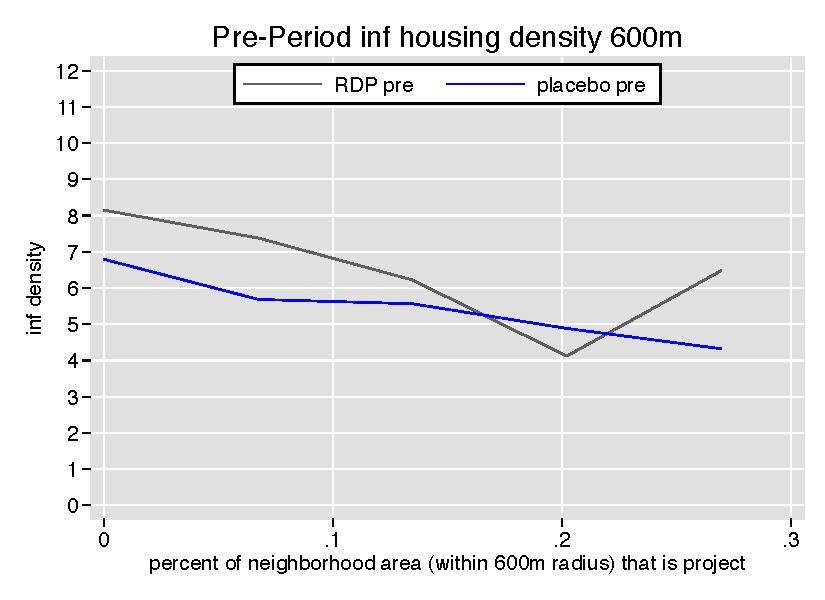
\includegraphics[width=\textwidth,trim={0.3cm .3cm 0.1cm 0cm}, clip=true]{figures/overlap_inf_600_total_pre.pdf}
        \end{subfigure}
        \vspace{-6mm}
        %\vspace{2mm}
        \begin{subfigure}[b]{0.495\textwidth}
            \centering
            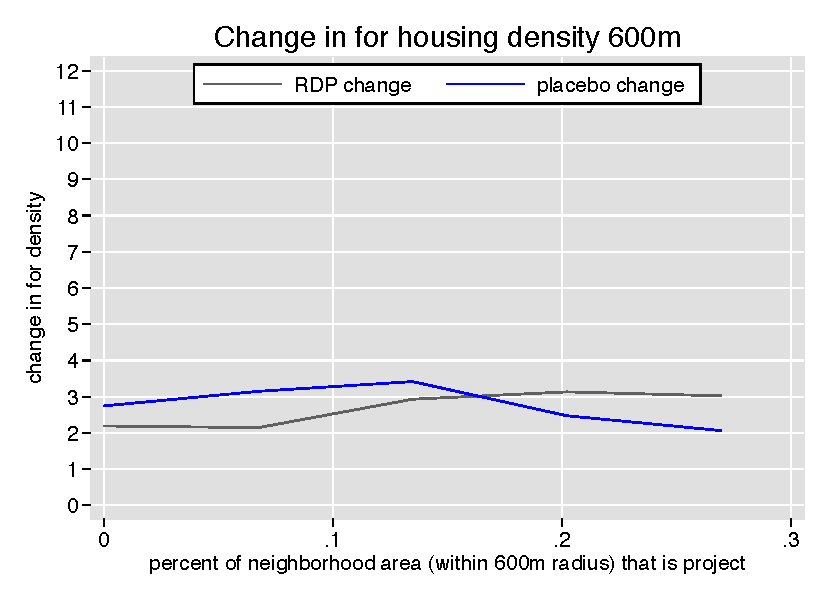
\includegraphics[width=\textwidth,trim={0.3cm .3cm 0.1cm 0cm}, clip=true]{figures/change_for_600_total.pdf}
        \end{subfigure}
        \hfill
        \begin{subfigure}[b]{0.495\textwidth}  
            \centering 
            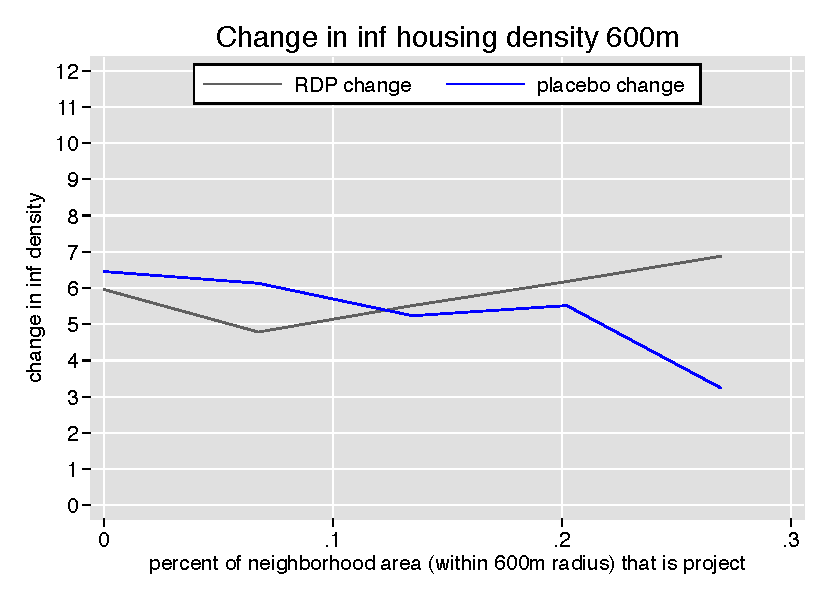
\includegraphics[width=\textwidth,trim={0.3cm .3cm 0.1cm 0cm}, clip=true]{figures/change_inf_600_total.pdf}
        \end{subfigure}
        \vspace{-6mm}
    \end{figure*} 


\begin{figure*}
        %\vspace{2mm}
        \begin{subfigure}[b]{0.495\textwidth}
            \centering
            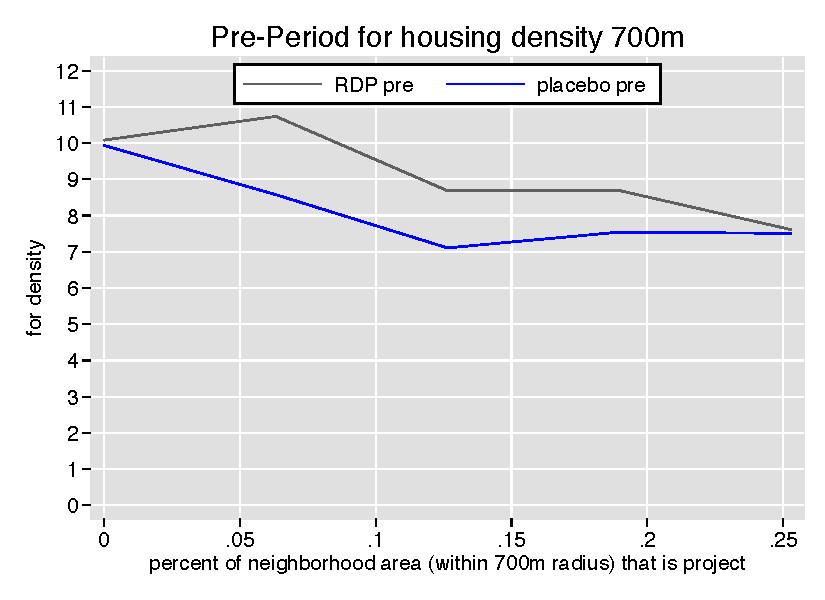
\includegraphics[width=\textwidth,trim={0.3cm .3cm 0.1cm 0cm}, clip=true]{figures/overlap_for_700_total_pre.pdf}
        \end{subfigure}
        \hfill
        \begin{subfigure}[b]{0.495\textwidth}  
            \centering 
            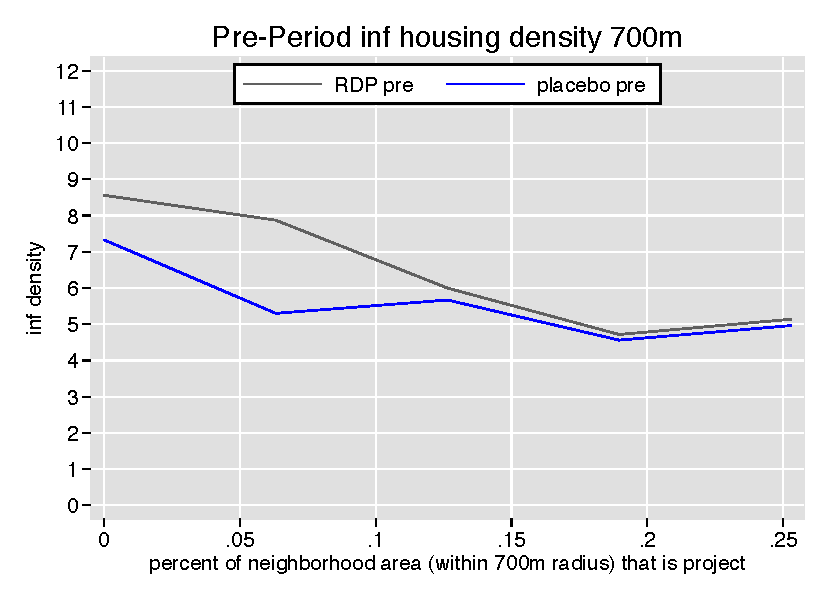
\includegraphics[width=\textwidth,trim={0.3cm .3cm 0.1cm 0cm}, clip=true]{figures/overlap_inf_700_total_pre.pdf}
        \end{subfigure}
        \vspace{-6mm}
        %\vspace{2mm}
        \begin{subfigure}[b]{0.495\textwidth}
            \centering
            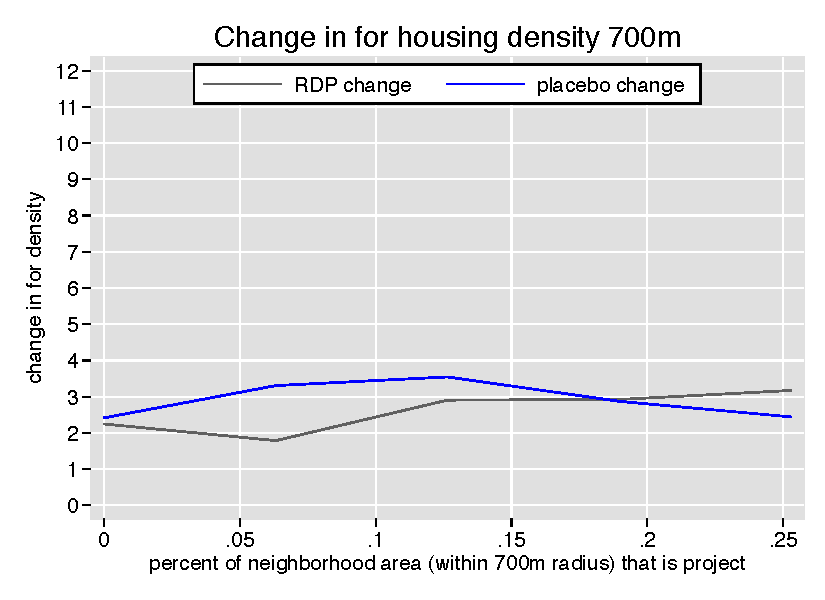
\includegraphics[width=\textwidth,trim={0.3cm .3cm 0.1cm 0cm}, clip=true]{figures/change_for_700_total.pdf}
        \end{subfigure}
        \hfill
        \begin{subfigure}[b]{0.495\textwidth}  
            \centering 
            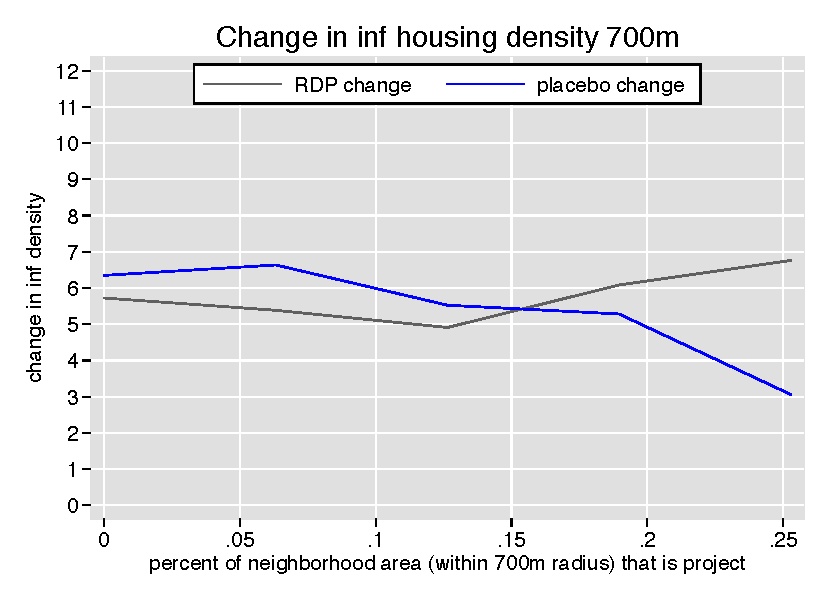
\includegraphics[width=\textwidth,trim={0.3cm .3cm 0.1cm 0cm}, clip=true]{figures/change_inf_700_total.pdf}
        \end{subfigure}
        \vspace{-6mm}
  \end{figure*} 



\pagebreak




\begin{figure*}
        %\vspace{2mm}
        \begin{subfigure}[b]{0.495\textwidth}
            \centering
            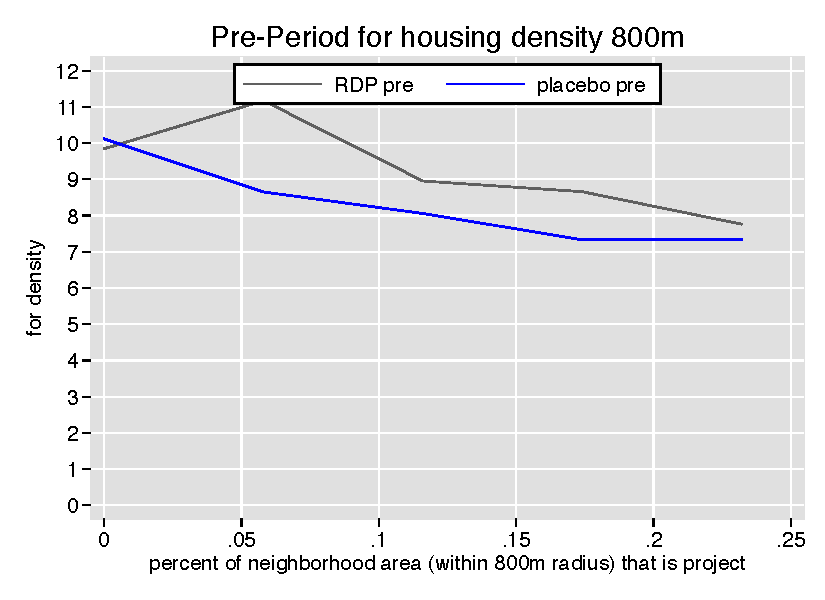
\includegraphics[width=\textwidth,trim={0.3cm .3cm 0.1cm 0cm}, clip=true]{figures/overlap_for_800_total_pre.pdf}
        \end{subfigure}
        \hfill
        \begin{subfigure}[b]{0.495\textwidth}  
            \centering 
            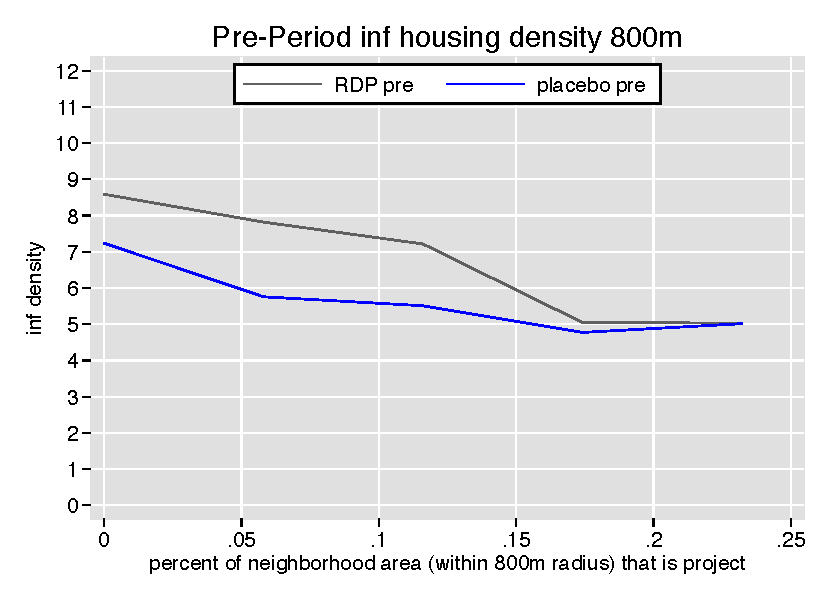
\includegraphics[width=\textwidth,trim={0.3cm .3cm 0.1cm 0cm}, clip=true]{figures/overlap_inf_800_total_pre.pdf}
        \end{subfigure}
        \vspace{-6mm}
        %\vspace{2mm}
        \begin{subfigure}[b]{0.495\textwidth}
            \centering
            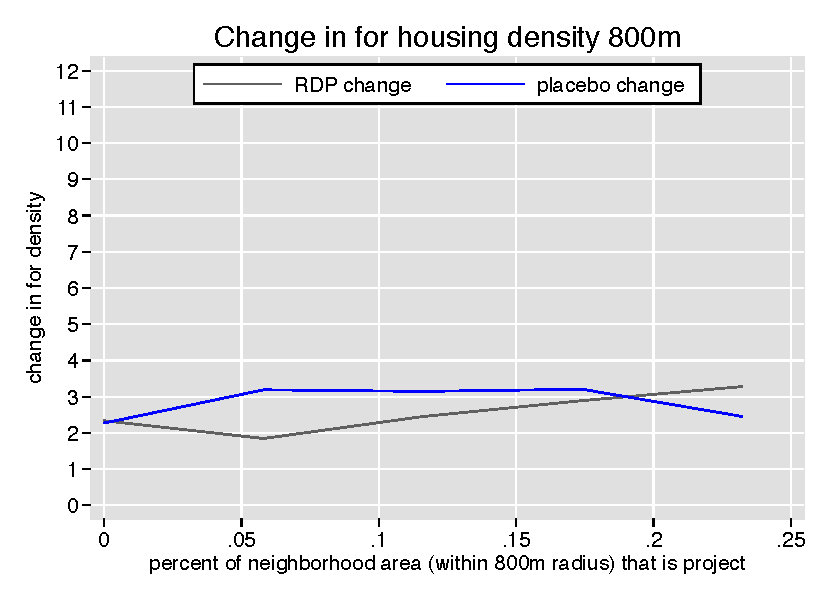
\includegraphics[width=\textwidth,trim={0.3cm .3cm 0.1cm 0cm}, clip=true]{figures/change_for_800_total.pdf}
        \end{subfigure}
        \hfill
        \begin{subfigure}[b]{0.495\textwidth}  
            \centering 
            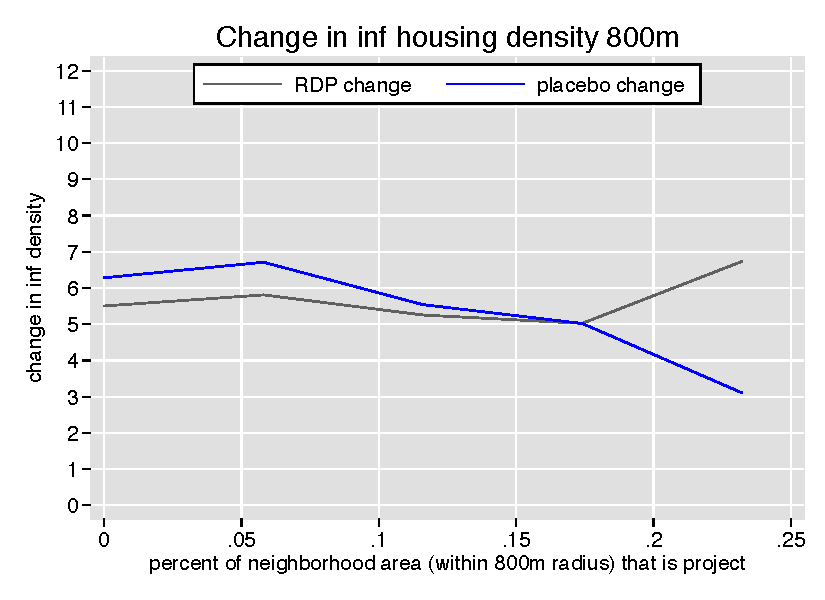
\includegraphics[width=\textwidth,trim={0.3cm .3cm 0.1cm 0cm}, clip=true]{figures/change_inf_800_total.pdf}
        \end{subfigure}
        \vspace{-6mm}
    \end{figure*} 


\begin{figure*}
        %\vspace{2mm}
        \begin{subfigure}[b]{0.495\textwidth}
            \centering
            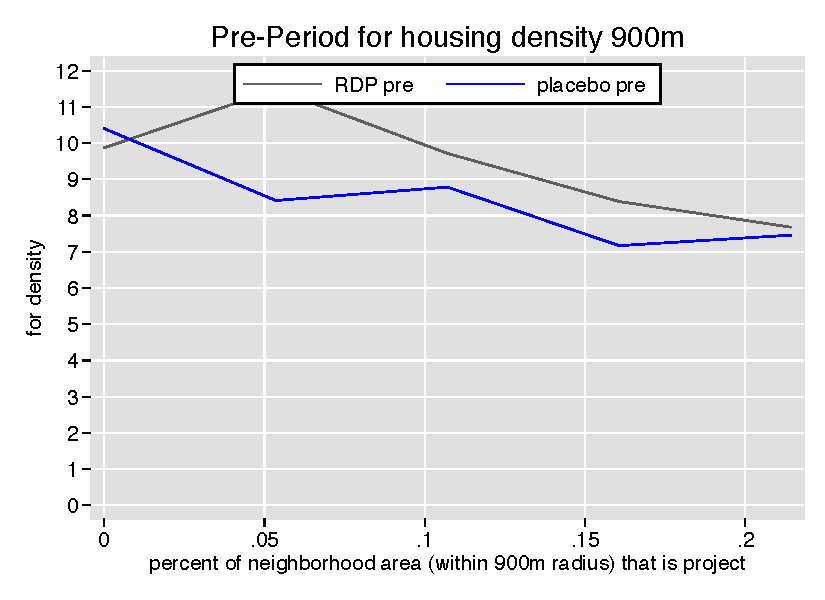
\includegraphics[width=\textwidth,trim={0.3cm .3cm 0.1cm 0cm}, clip=true]{figures/overlap_for_900_total_pre.pdf}
        \end{subfigure}
        \hfill
        \begin{subfigure}[b]{0.495\textwidth}  
            \centering 
            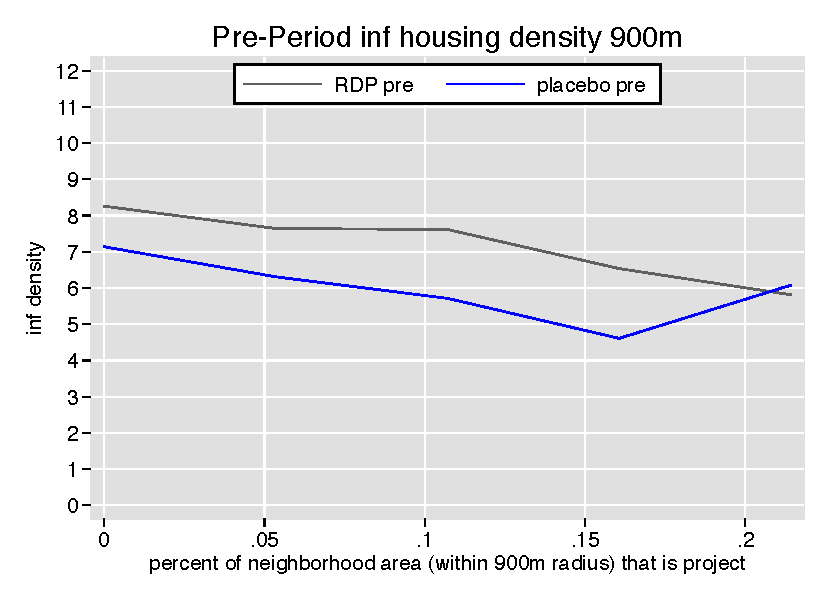
\includegraphics[width=\textwidth,trim={0.3cm .3cm 0.1cm 0cm}, clip=true]{figures/overlap_inf_900_total_pre.pdf}
        \end{subfigure}
        \vspace{-6mm}
        %\vspace{2mm}
        \begin{subfigure}[b]{0.495\textwidth}
            \centering
            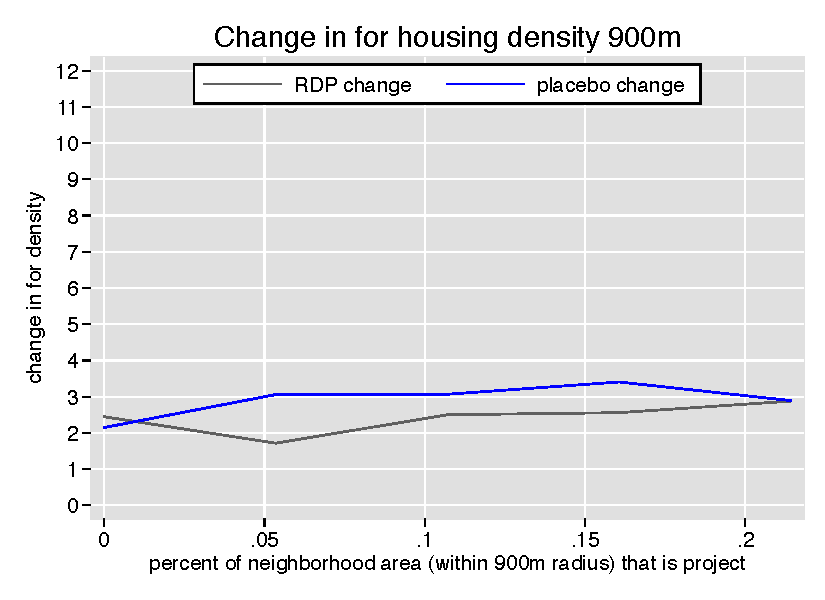
\includegraphics[width=\textwidth,trim={0.3cm .3cm 0.1cm 0cm}, clip=true]{figures/change_for_900_total.pdf}
        \end{subfigure}
        \hfill
        \begin{subfigure}[b]{0.495\textwidth}  
            \centering 
            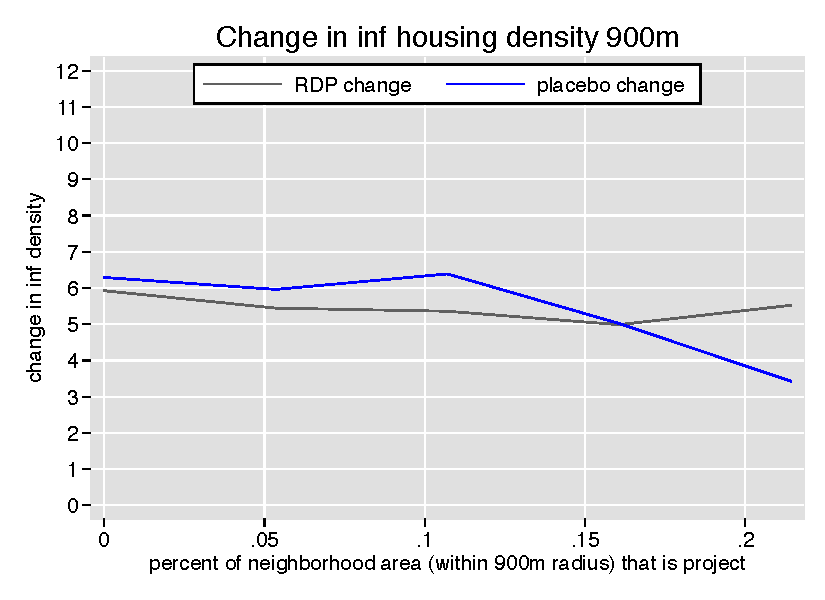
\includegraphics[width=\textwidth,trim={0.3cm .3cm 0.1cm 0cm}, clip=true]{figures/change_inf_900_total.pdf}
        \end{subfigure}
        \vspace{-6mm}
  \end{figure*} 



\pagebreak





\begin{figure*}
        %\vspace{2mm}
        \begin{subfigure}[b]{0.495\textwidth}
            \centering
            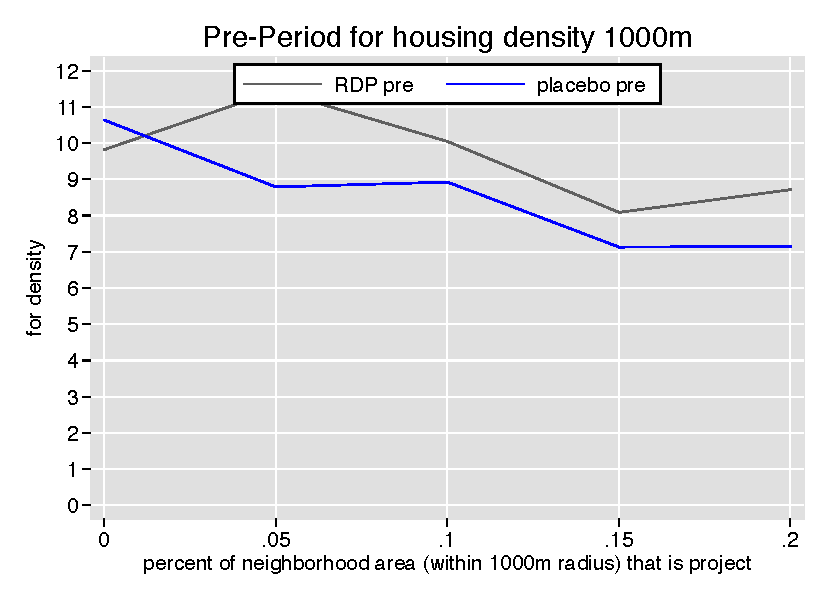
\includegraphics[width=\textwidth,trim={0.3cm .3cm 0.1cm 0cm}, clip=true]{figures/overlap_for_1000_total_pre.pdf}
        \end{subfigure}
        \hfill
        \begin{subfigure}[b]{0.495\textwidth}  
            \centering 
            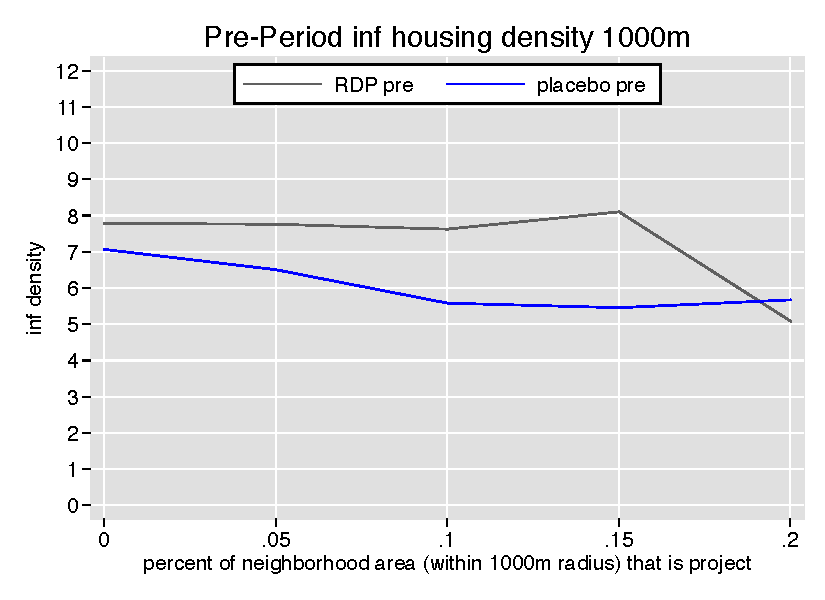
\includegraphics[width=\textwidth,trim={0.3cm .3cm 0.1cm 0cm}, clip=true]{figures/overlap_inf_1000_total_pre.pdf}
        \end{subfigure}
        \vspace{-6mm}
        %\vspace{2mm}
        \begin{subfigure}[b]{0.495\textwidth}
            \centering
            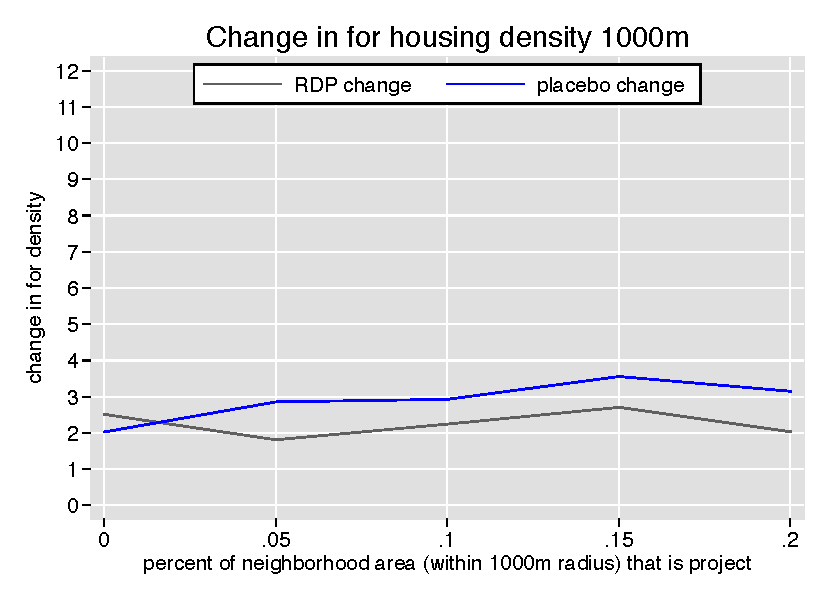
\includegraphics[width=\textwidth,trim={0.3cm .3cm 0.1cm 0cm}, clip=true]{figures/change_for_1000_total.pdf}
        \end{subfigure}
        \hfill
        \begin{subfigure}[b]{0.495\textwidth}  
            \centering 
            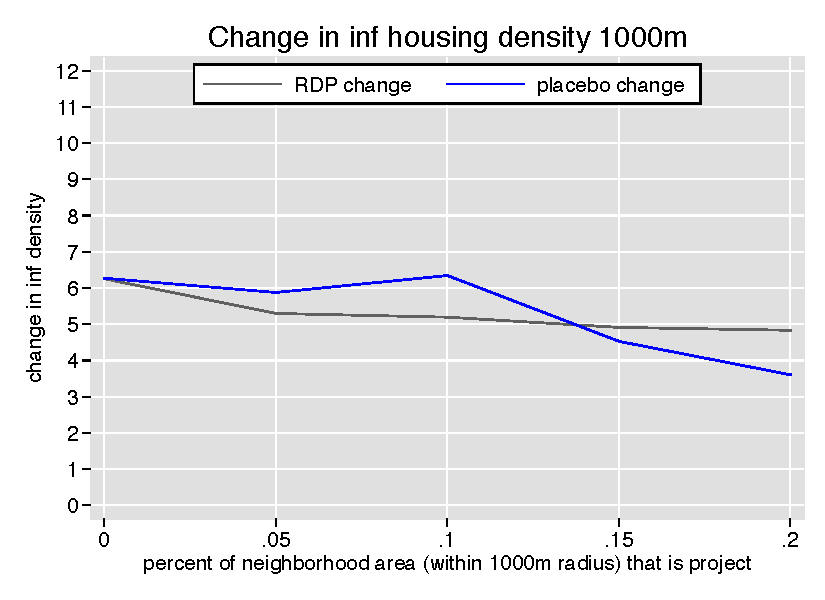
\includegraphics[width=\textwidth,trim={0.3cm .3cm 0.1cm 0cm}, clip=true]{figures/change_inf_1000_total.pdf}
        \end{subfigure}
        \vspace{-6mm}
    \end{figure*} 


\begin{figure*}
        %\vspace{2mm}
        \begin{subfigure}[b]{0.495\textwidth}
            \centering
            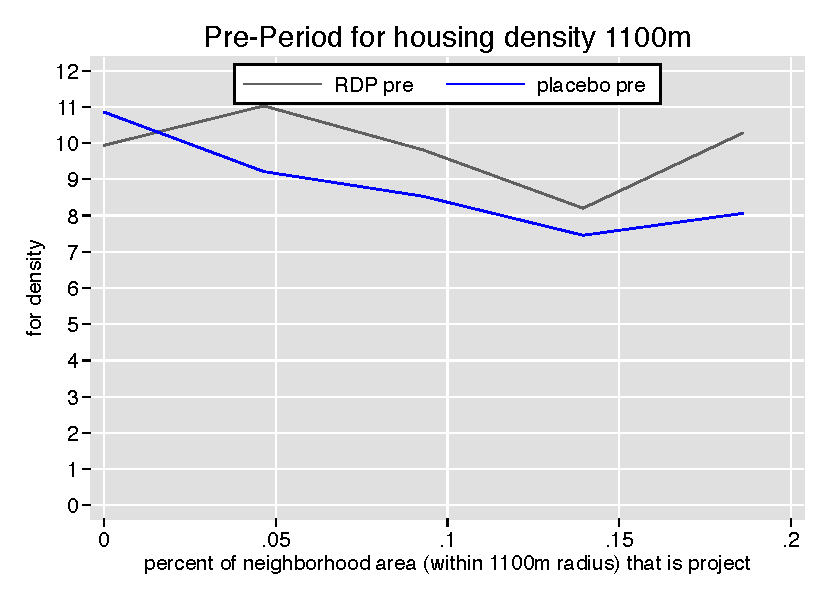
\includegraphics[width=\textwidth,trim={0.3cm .3cm 0.1cm 0cm}, clip=true]{figures/overlap_for_1100_total_pre.pdf}
        \end{subfigure}
        \hfill
        \begin{subfigure}[b]{0.495\textwidth}  
            \centering 
            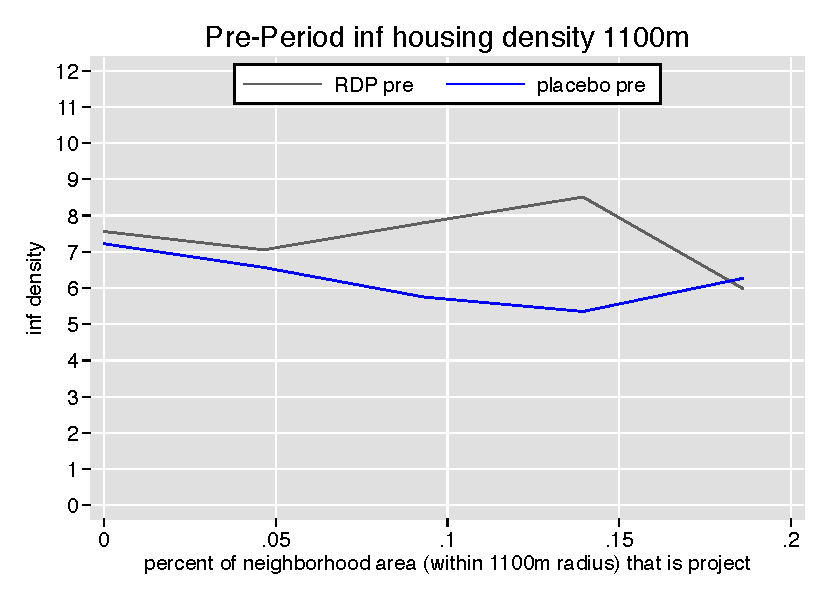
\includegraphics[width=\textwidth,trim={0.3cm .3cm 0.1cm 0cm}, clip=true]{figures/overlap_inf_1100_total_pre.pdf}
        \end{subfigure}
        \vspace{-6mm}
        %\vspace{2mm}
        \begin{subfigure}[b]{0.495\textwidth}
            \centering
            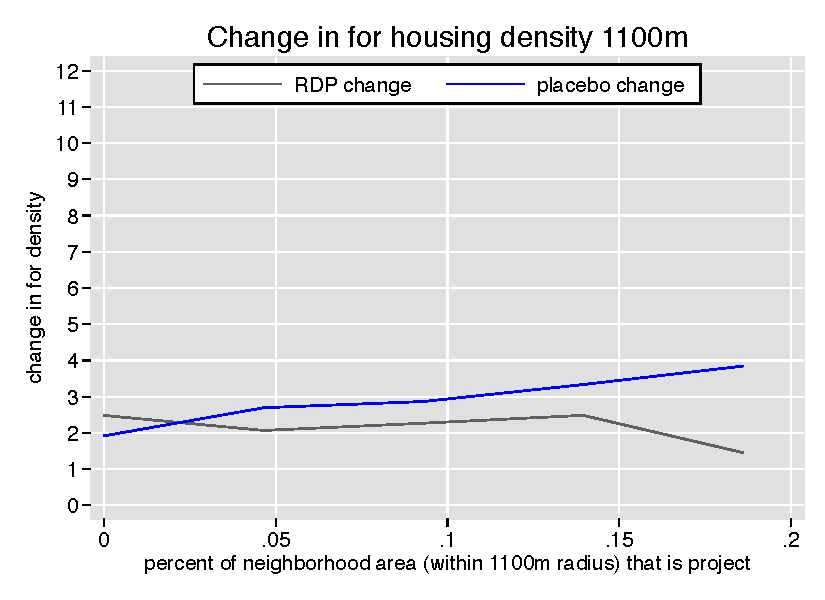
\includegraphics[width=\textwidth,trim={0.3cm .3cm 0.1cm 0cm}, clip=true]{figures/change_for_1100_total.pdf}
        \end{subfigure}
        \hfill
        \begin{subfigure}[b]{0.495\textwidth}  
            \centering 
            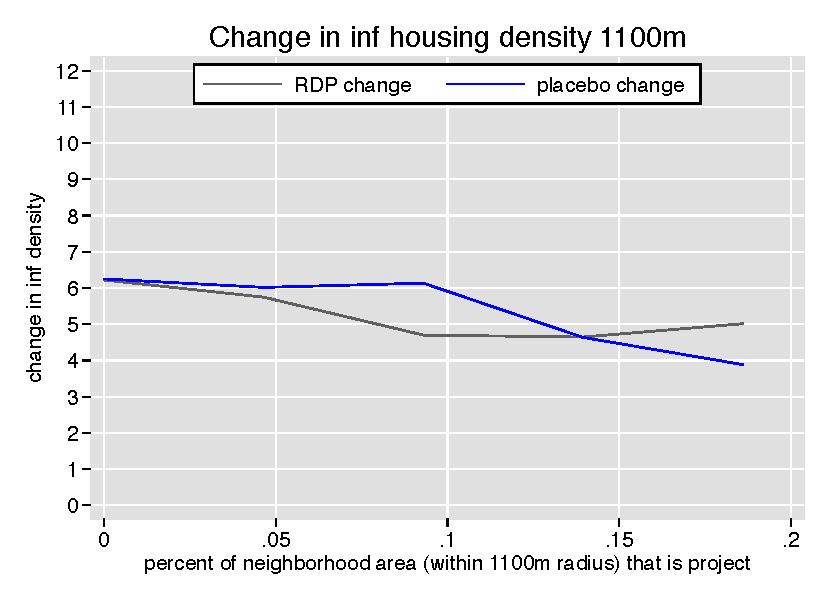
\includegraphics[width=\textwidth,trim={0.3cm .3cm 0.1cm 0cm}, clip=true]{figures/change_inf_1100_total.pdf}
        \end{subfigure}
        \vspace{-6mm}
  \end{figure*} 



\pagebreak





\begin{figure*}
        %\vspace{2mm}
        \begin{subfigure}[b]{0.495\textwidth}
            \centering
            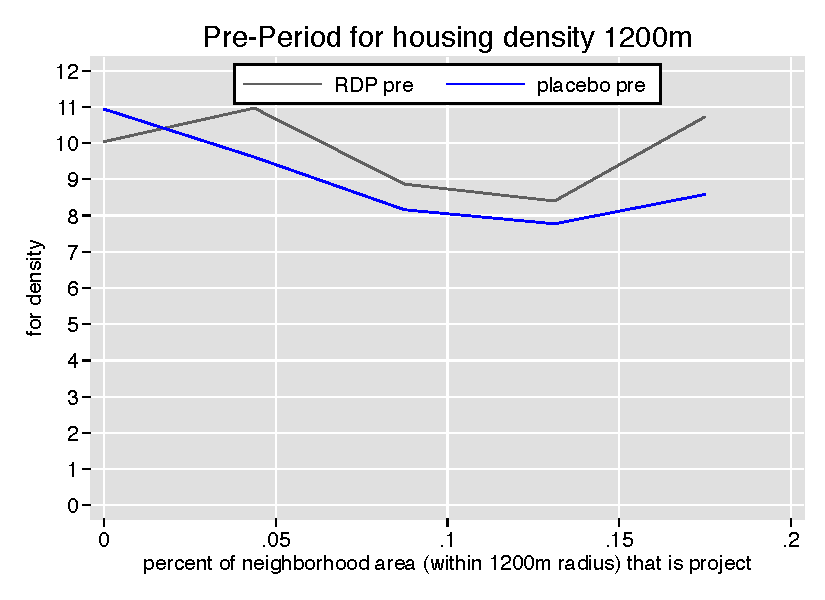
\includegraphics[width=\textwidth,trim={0.3cm .3cm 0.1cm 0cm}, clip=true]{figures/overlap_for_1200_total_pre.pdf}
        \end{subfigure}
        \hfill
        \begin{subfigure}[b]{0.495\textwidth}  
            \centering 
            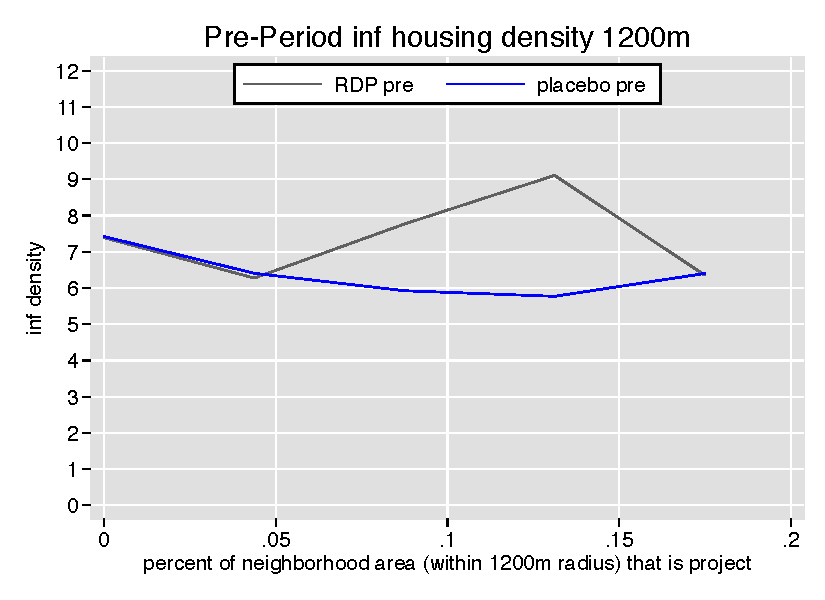
\includegraphics[width=\textwidth,trim={0.3cm .3cm 0.1cm 0cm}, clip=true]{figures/overlap_inf_1200_total_pre.pdf}
        \end{subfigure}
        \vspace{-6mm}
        %\vspace{2mm}
        \begin{subfigure}[b]{0.495\textwidth}
            \centering
            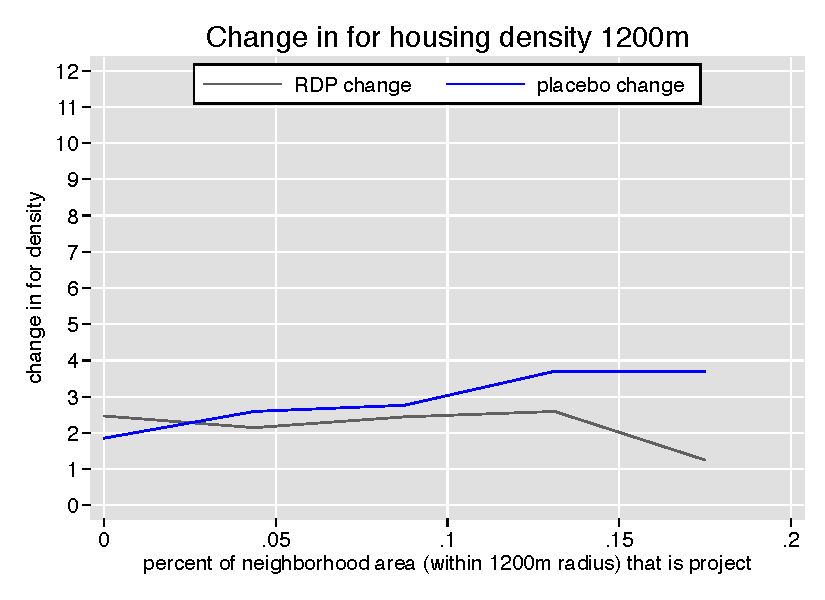
\includegraphics[width=\textwidth,trim={0.3cm .3cm 0.1cm 0cm}, clip=true]{figures/change_for_1200_total.pdf}
        \end{subfigure}
        \hfill
        \begin{subfigure}[b]{0.495\textwidth}  
            \centering 
            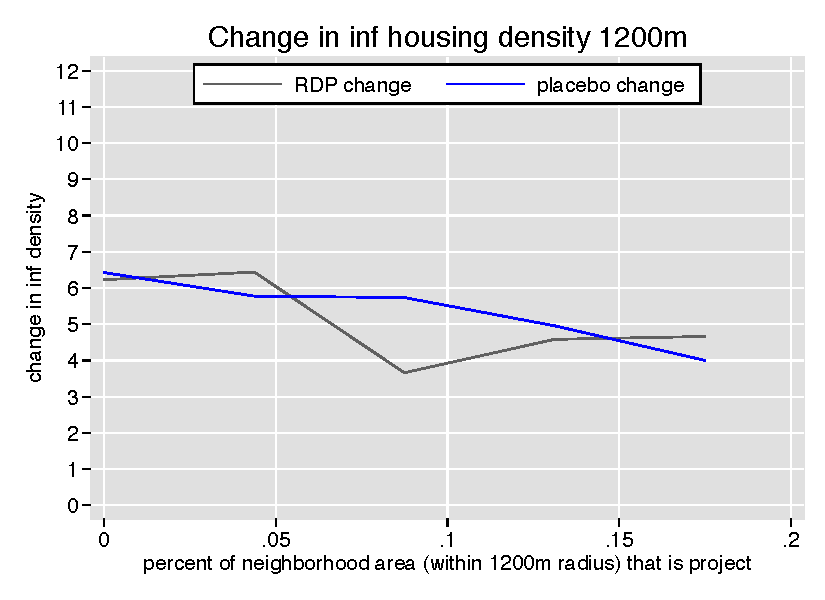
\includegraphics[width=\textwidth,trim={0.3cm .3cm 0.1cm 0cm}, clip=true]{figures/change_inf_1200_total.pdf}
        \end{subfigure}
        \vspace{-6mm}
    \end{figure*} 







% \pagebreak

% \section{ROBUSTNESS : Excluding any RDP (placebo) points that overlap with placebo (RDP) Projects}

% \begin{figure*}
%         %\vspace{2mm}
%         \begin{subfigure}[b]{0.495\textwidth}
%             \centering
%             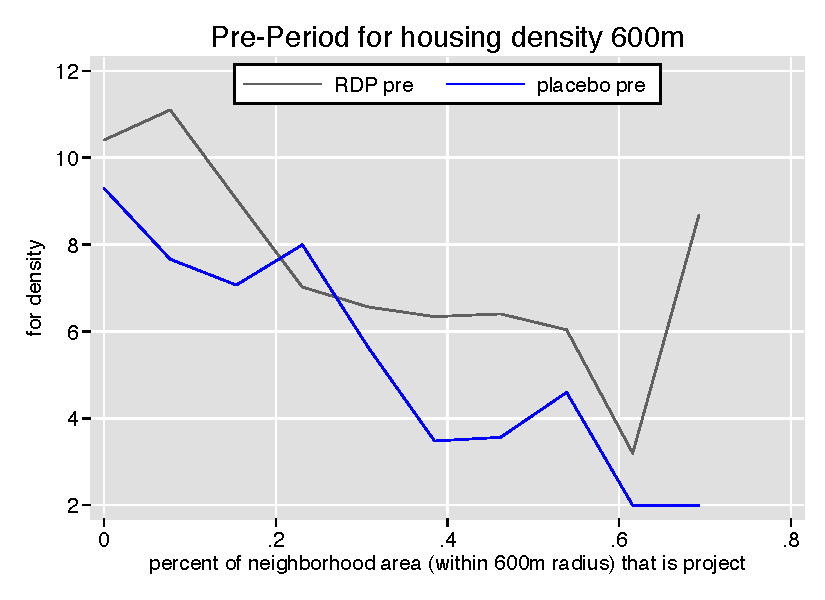
\includegraphics[width=\textwidth,trim={0.3cm .3cm 0.1cm 0cm}, clip=true]{figures/overlap_for_600_local_pre.pdf}
%         \end{subfigure}
%         \hfill
%         \begin{subfigure}[b]{0.495\textwidth}  
%             \centering 
%             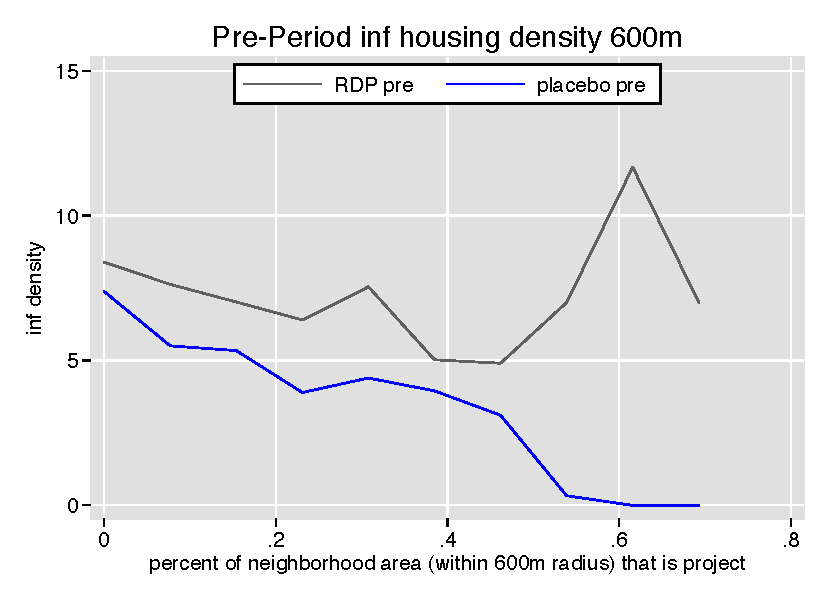
\includegraphics[width=\textwidth,trim={0.3cm .3cm 0.1cm 0cm}, clip=true]{figures/overlap_inf_600_local_pre.pdf}
%         \end{subfigure}
%         \vspace{-6mm}
%         %\vspace{2mm}
%         \begin{subfigure}[b]{0.495\textwidth}
%             \centering
%             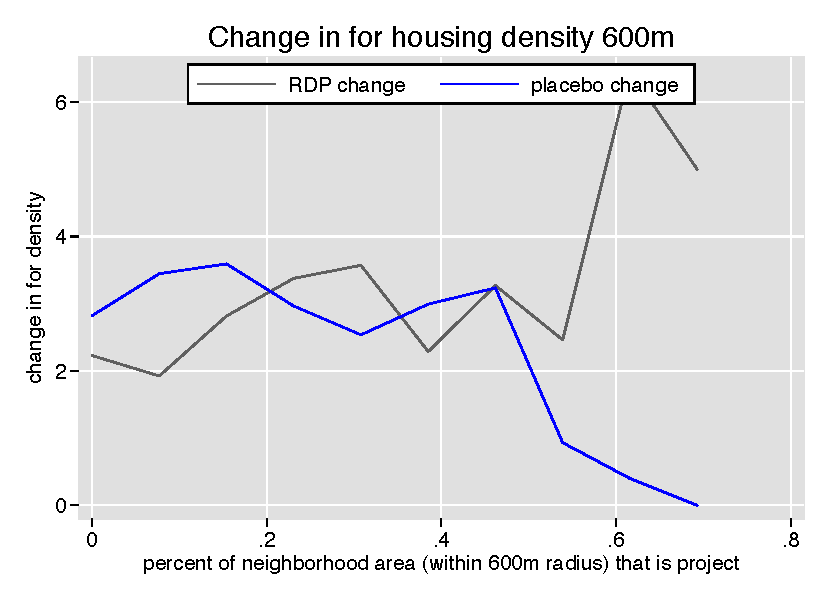
\includegraphics[width=\textwidth,trim={0.3cm .3cm 0.1cm 0cm}, clip=true]{figures/change_for_600_local.pdf}
%         \end{subfigure}
%         \hfill
%         \begin{subfigure}[b]{0.495\textwidth}  
%             \centering 
%             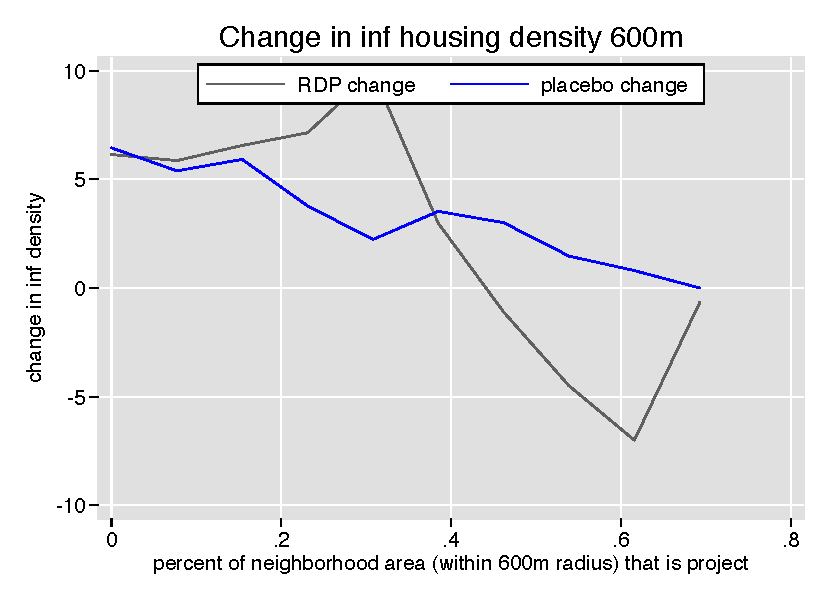
\includegraphics[width=\textwidth,trim={0.3cm .3cm 0.1cm 0cm}, clip=true]{figures/change_inf_600_local.pdf}
%         \end{subfigure}
%         \vspace{-6mm}
%     \end{figure*} 


% \begin{figure*}
%         %\vspace{2mm}
%         \begin{subfigure}[b]{0.495\textwidth}
%             \centering
%             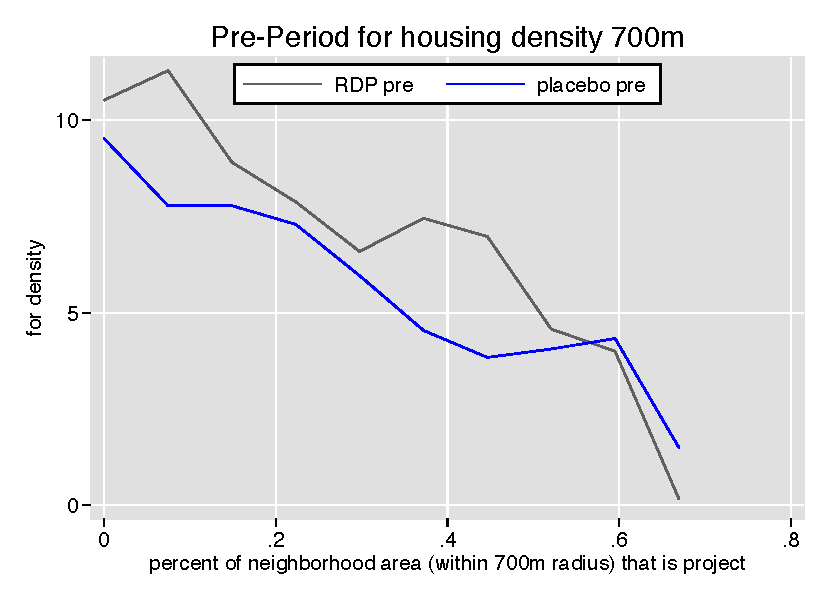
\includegraphics[width=\textwidth,trim={0.3cm .3cm 0.1cm 0cm}, clip=true]{figures/overlap_for_700_local_pre.pdf}
%         \end{subfigure}
%         \hfill
%         \begin{subfigure}[b]{0.495\textwidth}  
%             \centering 
%             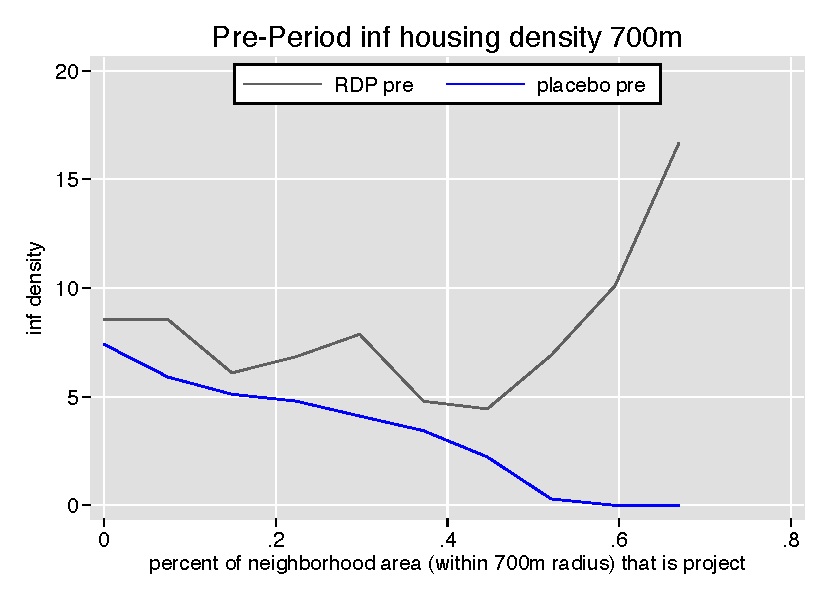
\includegraphics[width=\textwidth,trim={0.3cm .3cm 0.1cm 0cm}, clip=true]{figures/overlap_inf_700_local_pre.pdf}
%         \end{subfigure}
%         \vspace{-6mm}
%         %\vspace{2mm}
%         \begin{subfigure}[b]{0.495\textwidth}
%             \centering
%             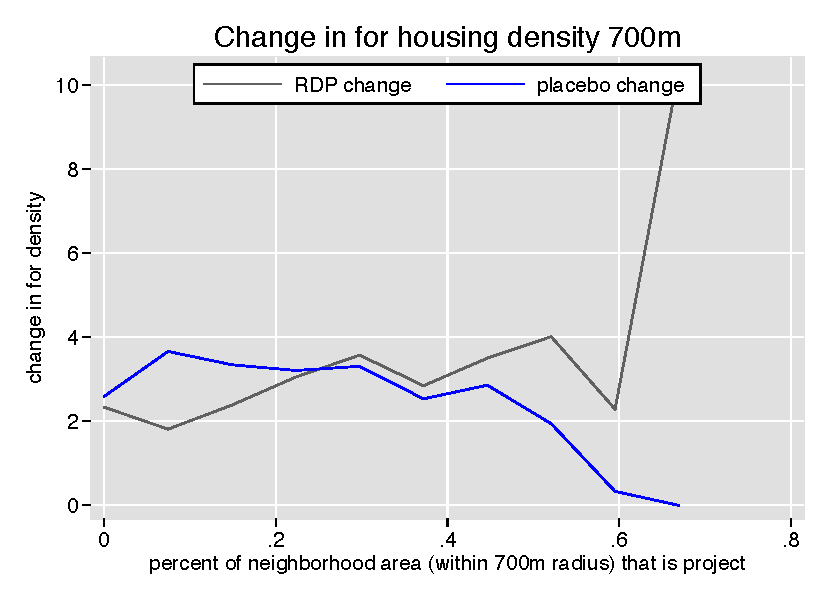
\includegraphics[width=\textwidth,trim={0.3cm .3cm 0.1cm 0cm}, clip=true]{figures/change_for_700_local.pdf}
%         \end{subfigure}
%         \hfill
%         \begin{subfigure}[b]{0.495\textwidth}  
%             \centering 
%             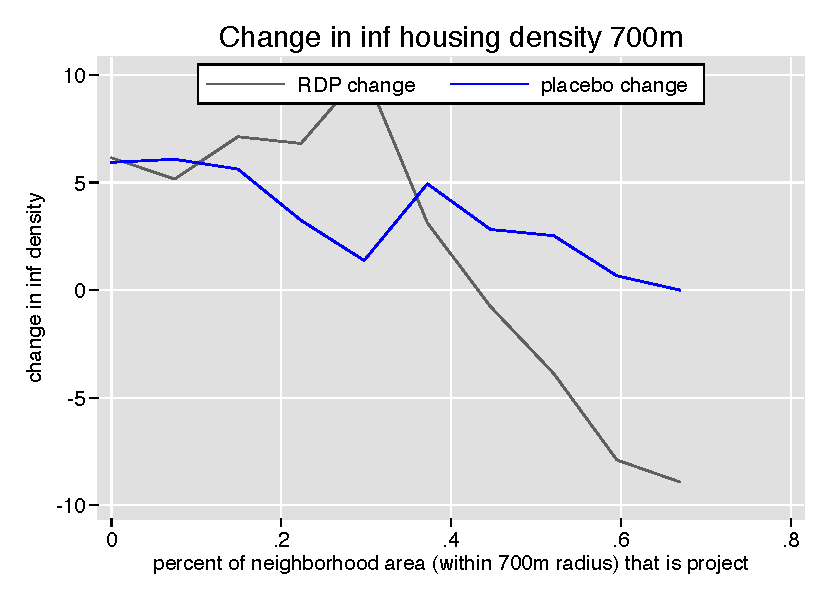
\includegraphics[width=\textwidth,trim={0.3cm .3cm 0.1cm 0cm}, clip=true]{figures/change_inf_700_local.pdf}
%         \end{subfigure}
%         \vspace{-6mm}
%   \end{figure*} 



% \pagebreak




% \begin{figure*}
%         %\vspace{2mm}
%         \begin{subfigure}[b]{0.495\textwidth}
%             \centering
%             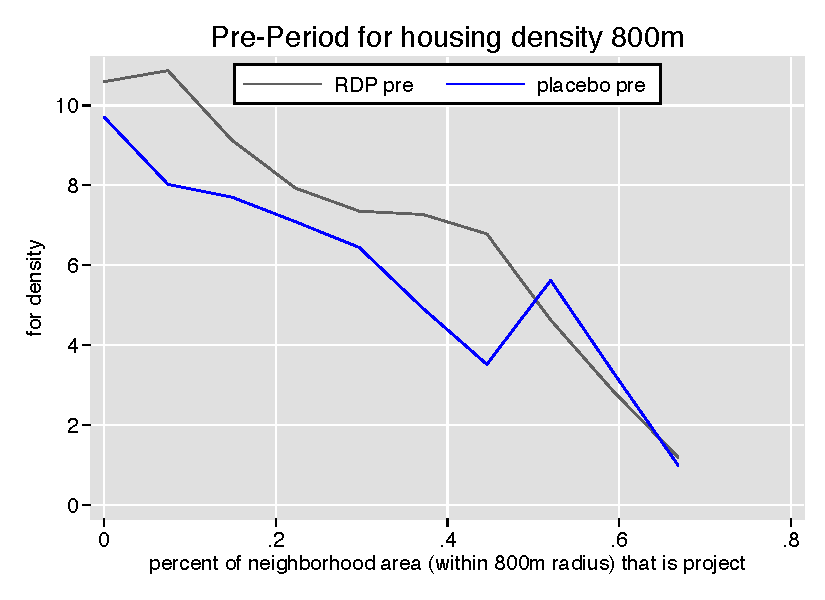
\includegraphics[width=\textwidth,trim={0.3cm .3cm 0.1cm 0cm}, clip=true]{figures/overlap_for_800_local_pre.pdf}
%         \end{subfigure}
%         \hfill
%         \begin{subfigure}[b]{0.495\textwidth}  
%             \centering 
%             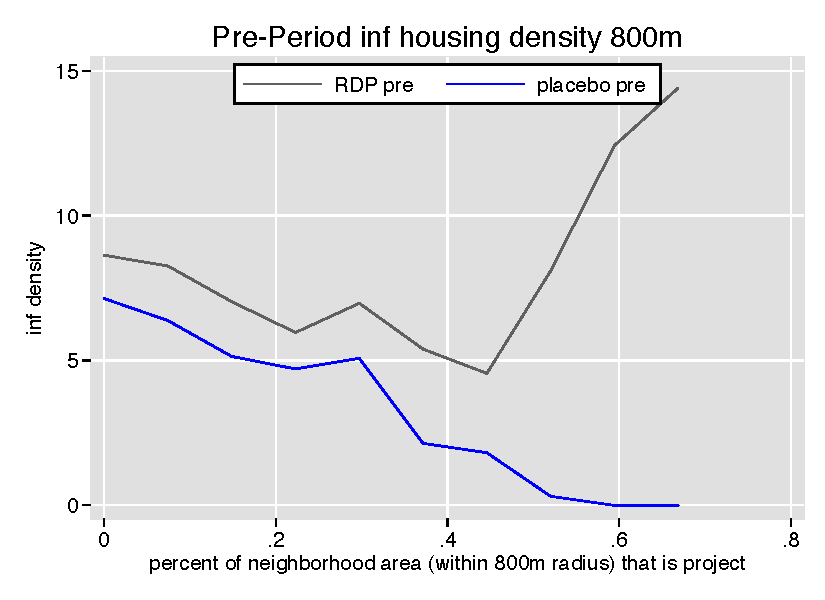
\includegraphics[width=\textwidth,trim={0.3cm .3cm 0.1cm 0cm}, clip=true]{figures/overlap_inf_800_local_pre.pdf}
%         \end{subfigure}
%         \vspace{-6mm}
%         %\vspace{2mm}
%         \begin{subfigure}[b]{0.495\textwidth}
%             \centering
%             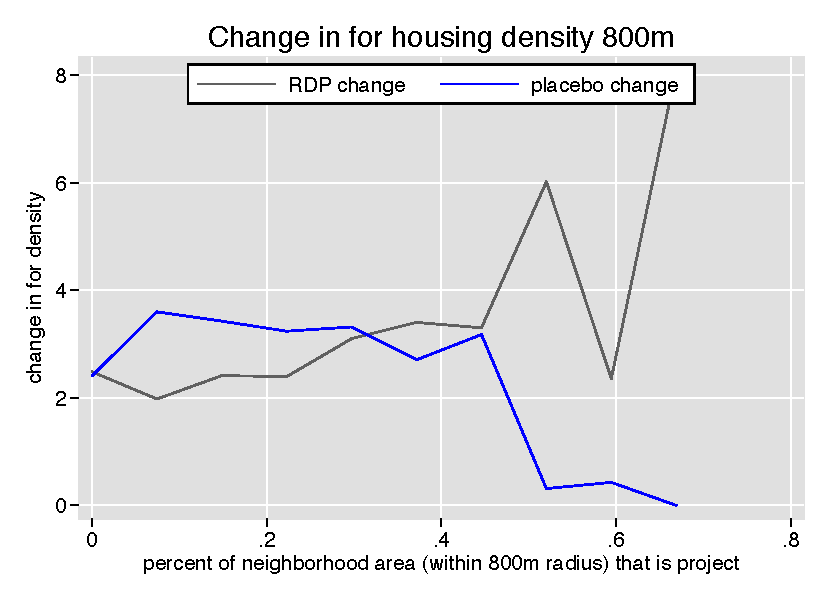
\includegraphics[width=\textwidth,trim={0.3cm .3cm 0.1cm 0cm}, clip=true]{figures/change_for_800_local.pdf}
%         \end{subfigure}
%         \hfill
%         \begin{subfigure}[b]{0.495\textwidth}  
%             \centering 
%             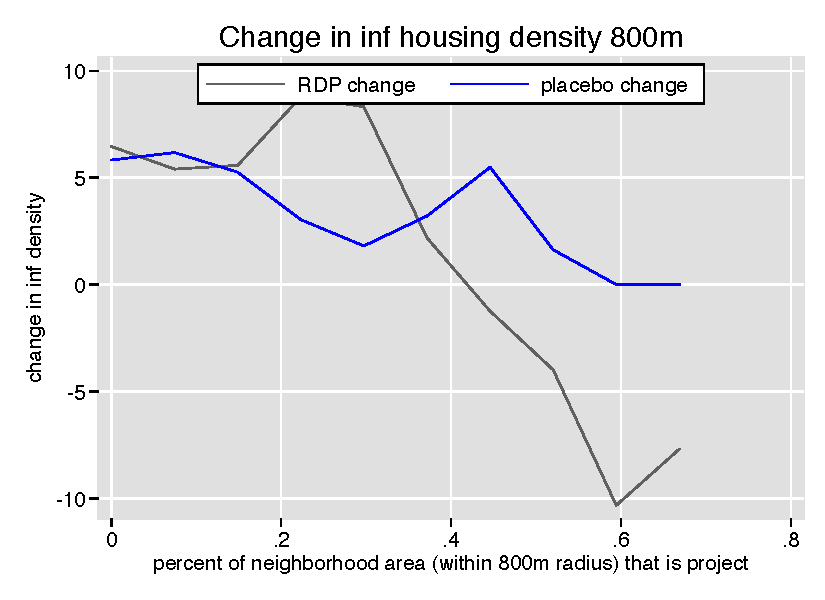
\includegraphics[width=\textwidth,trim={0.3cm .3cm 0.1cm 0cm}, clip=true]{figures/change_inf_800_local.pdf}
%         \end{subfigure}
%         \vspace{-6mm}
%     \end{figure*} 


% \begin{figure*}
%         %\vspace{2mm}
%         \begin{subfigure}[b]{0.495\textwidth}
%             \centering
%             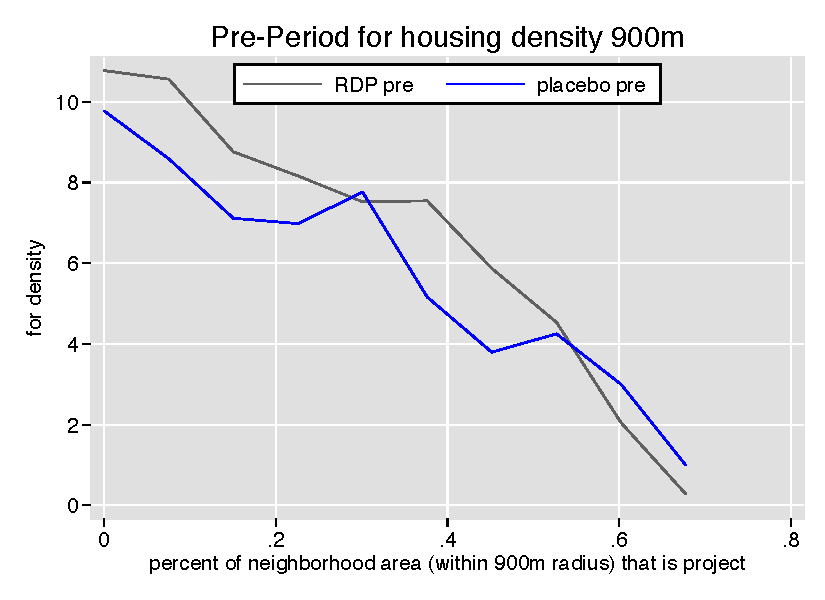
\includegraphics[width=\textwidth,trim={0.3cm .3cm 0.1cm 0cm}, clip=true]{figures/overlap_for_900_local_pre.pdf}
%         \end{subfigure}
%         \hfill
%         \begin{subfigure}[b]{0.495\textwidth}  
%             \centering 
%             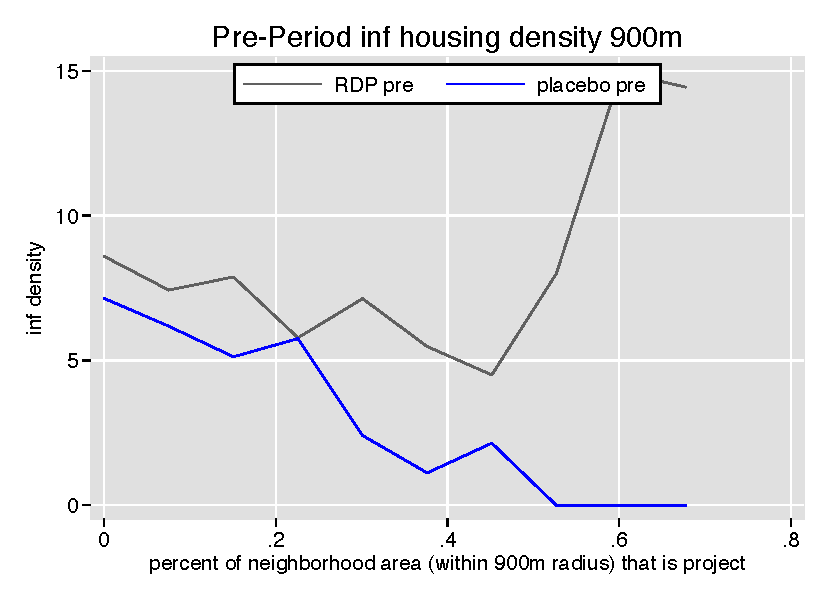
\includegraphics[width=\textwidth,trim={0.3cm .3cm 0.1cm 0cm}, clip=true]{figures/overlap_inf_900_local_pre.pdf}
%         \end{subfigure}
%         \vspace{-6mm}
%         %\vspace{2mm}
%         \begin{subfigure}[b]{0.495\textwidth}
%             \centering
%             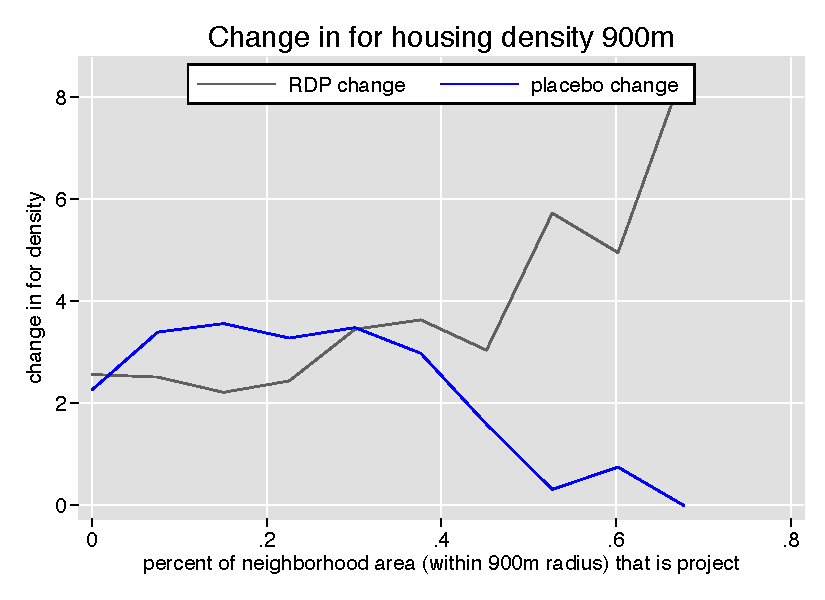
\includegraphics[width=\textwidth,trim={0.3cm .3cm 0.1cm 0cm}, clip=true]{figures/change_for_900_local.pdf}
%         \end{subfigure}
%         \hfill
%         \begin{subfigure}[b]{0.495\textwidth}  
%             \centering 
%             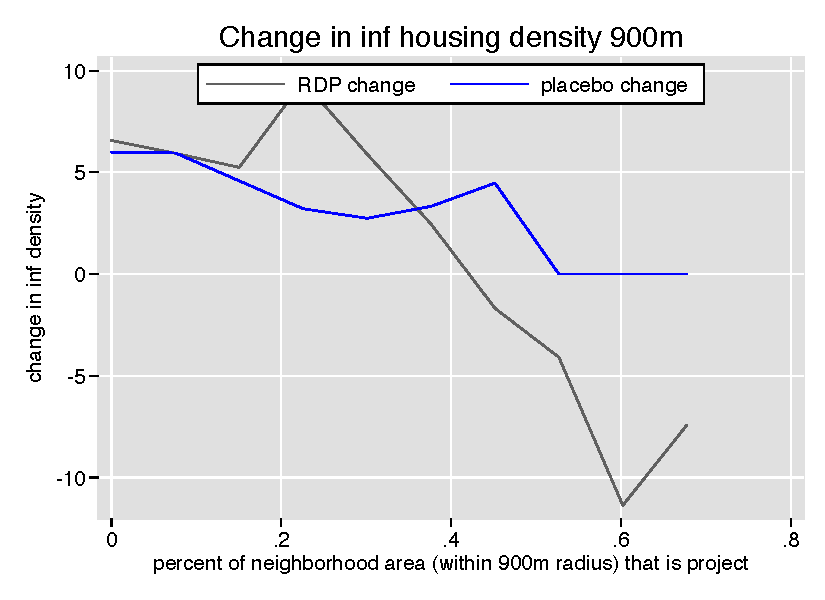
\includegraphics[width=\textwidth,trim={0.3cm .3cm 0.1cm 0cm}, clip=true]{figures/change_inf_900_local.pdf}
%         \end{subfigure}
%         \vspace{-6mm}
%   \end{figure*} 



% \pagebreak





% \begin{figure*}
%         %\vspace{2mm}
%         \begin{subfigure}[b]{0.495\textwidth}
%             \centering
%             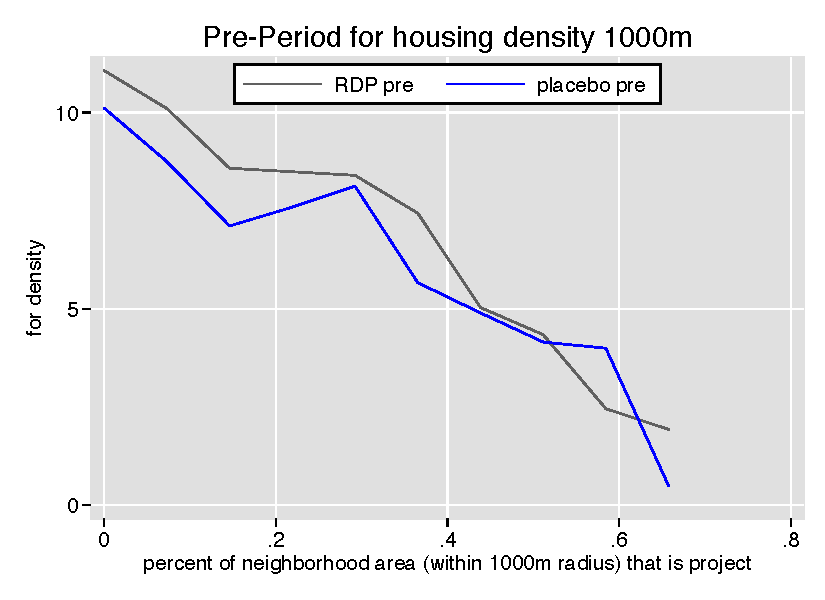
\includegraphics[width=\textwidth,trim={0.3cm .3cm 0.1cm 0cm}, clip=true]{figures/overlap_for_1000_local_pre.pdf}
%         \end{subfigure}
%         \hfill
%         \begin{subfigure}[b]{0.495\textwidth}  
%             \centering 
%             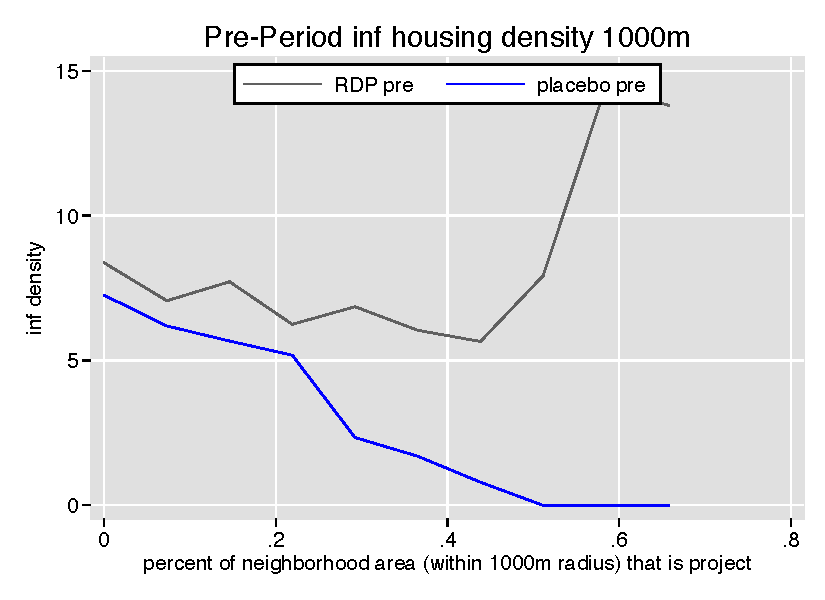
\includegraphics[width=\textwidth,trim={0.3cm .3cm 0.1cm 0cm}, clip=true]{figures/overlap_inf_1000_local_pre.pdf}
%         \end{subfigure}
%         \vspace{-6mm}
%         %\vspace{2mm}
%         \begin{subfigure}[b]{0.495\textwidth}
%             \centering
%             \includegraphics[width=\textwidth,trim={0.3cm .3cm 0.1cm 0cm}, clip=true]{figures/change_for_1000_local.pdf}
%         \end{subfigure}
%         \hfill
%         \begin{subfigure}[b]{0.495\textwidth}  
%             \centering 
%             \includegraphics[width=\textwidth,trim={0.3cm .3cm 0.1cm 0cm}, clip=true]{figures/change_inf_1000_local.pdf}
%         \end{subfigure}
%         \vspace{-6mm}
%     \end{figure*} 


% \begin{figure*}
%         %\vspace{2mm}
%         \begin{subfigure}[b]{0.495\textwidth}
%             \centering
%             \includegraphics[width=\textwidth,trim={0.3cm .3cm 0.1cm 0cm}, clip=true]{figures/overlap_for_1100_local_pre.pdf}
%         \end{subfigure}
%         \hfill
%         \begin{subfigure}[b]{0.495\textwidth}  
%             \centering 
%             \includegraphics[width=\textwidth,trim={0.3cm .3cm 0.1cm 0cm}, clip=true]{figures/overlap_inf_1100_local_pre.pdf}
%         \end{subfigure}
%         \vspace{-6mm}
%         %\vspace{2mm}
%         \begin{subfigure}[b]{0.495\textwidth}
%             \centering
%             \includegraphics[width=\textwidth,trim={0.3cm .3cm 0.1cm 0cm}, clip=true]{figures/change_for_1100_local.pdf}
%         \end{subfigure}
%         \hfill
%         \begin{subfigure}[b]{0.495\textwidth}  
%             \centering 
%             \includegraphics[width=\textwidth,trim={0.3cm .3cm 0.1cm 0cm}, clip=true]{figures/change_inf_1100_local.pdf}
%         \end{subfigure}
%         \vspace{-6mm}
%   \end{figure*} 



% \pagebreak





% \begin{figure*}
%         %\vspace{2mm}
%         \begin{subfigure}[b]{0.495\textwidth}
%             \centering
%             \includegraphics[width=\textwidth,trim={0.3cm .3cm 0.1cm 0cm}, clip=true]{figures/overlap_for_1200_local_pre.pdf}
%         \end{subfigure}
%         \hfill
%         \begin{subfigure}[b]{0.495\textwidth}  
%             \centering 
%             \includegraphics[width=\textwidth,trim={0.3cm .3cm 0.1cm 0cm}, clip=true]{figures/overlap_inf_1200_local_pre.pdf}
%         \end{subfigure}
%         \vspace{-6mm}
%         %\vspace{2mm}
%         \begin{subfigure}[b]{0.495\textwidth}
%             \centering
%             \includegraphics[width=\textwidth,trim={0.3cm .3cm 0.1cm 0cm}, clip=true]{figures/change_for_1200_local.pdf}
%         \end{subfigure}
%         \hfill
%         \begin{subfigure}[b]{0.495\textwidth}  
%             \centering 
%             \includegraphics[width=\textwidth,trim={0.3cm .3cm 0.1cm 0cm}, clip=true]{figures/change_inf_1200_local.pdf}
%         \end{subfigure}
%         \vspace{-6mm}
%     \end{figure*} 





% reg for post rdp_inside rdp_outside placebo_inside placebo_outside rdp_inside_post rdp_outside_post placebo_inside_post placebo_outside_post if cond2==1, cluster(cluster_reg)

% \pagebreak





% \begin{center}
% \begin{tikzpicture}


% \begin{scope}
%     \clip (1,1) rectangle (0,2);
%     \draw (1,1) circle(3.5cm);
%     %\draw (-1.5,0) -- (1.5,0);
% \end{scope}

% \draw (0,0) -- (2,0) -- (2,2) -- (0,2) -- (0,0);
% \node at (1,1) {RDP};
% \node at (1,1.5) {(1)};
% \node at (-1.5,1) {(4)};
% \node at (-5,1) {(7)};


% %\draw (1,1) circle (3.5cm);
% \draw (1,1) circle (7cm);

% \node at (2,3) {(3)};

% \node at (2,6) {(6)};

% \draw [thick,dash dot] (2,0) -- (4,0) -- (4,2) -- (2,2) -- (2,0);
% \node at (3,1) {Placebo};
% \node at (3,1.5) {(2)};
% \node at (5.5,1) {(5)};
% \node at (9,1) {(8)};

% \draw [thick,dash dot] (3,1) circle (3.5cm);
% \draw [thick,dash dot] (3,1) circle (7cm);

% \end{tikzpicture}
% \end{center}

% \begin{align*}
% Y = \underbrace{post}_{(1)-(8)} + (\underbrace{RDPinside}_{(1)} + \underbrace{RDPoutside}_{(3) + (4)} +   \underbrace{PCBinside}_{(2)} + \underbrace{PCBoutside}_{(3) + (5)})(1+post) + \epsilon
% \end{align*}
% reg for post rdp_inside rdp_outside placebo_inside placebo_outside rdp_inside_post rdp_outside_post placebo_inside_post placebo_outside_post if cond2==1, cluster(cluster_reg)

\end{document}


